% This is samplepaper.tex, a sample chapter demonstrating the
% LLNCS macro package for Springer Computer Science proceedings;
% Version 2.20 of 2017/10/04
%
\documentclass[runningheads]{llncs}
%
\usepackage{graphicx}
\usepackage{scrextend}
\usepackage{listings}
\usepackage{float}
\usepackage{subfig}
\lstloadlanguages{C,C++,csh,Java}
% Used for displaying a sample figure. If possible, figure files should
% be included in EPS format.
%
% If you use the hyperref package, please uncomment the following line
% to display URLs in blue roman font according to Springer's eBook style:
% \renewcommand\UrlFont{\color{blue}\rmfamily}

\begin{document}
%
\title{Virtual Reality and Logic Programming as Assistance in Architectural Design}
%
\titlerunning{VR and LP as Assistance in Architectural Design}
% If the paper title is too long for the running head, you can set
% an abbreviated paper title here
%
\author{Dominik Struga\l{}a, Krzysztof Walczak}
%
\authorrunning{Struga\l{}a, D., Walczak, K.} % abbreviated author list (for running head)
%
%
\institute{Pozna\'{n} University of Economics and Business,\\
Niepodleg\l{}o\'{s}ci 10, 61-875 Pozna\'{n}, Poland\\
\email{[strugala,walczak]@kti.ue.poznan.pl}\\
\texttt{http://www.kti.ue.poznan.pl/}
}
%
\maketitle              % typeset the header of the contribution
%
\begin{abstract}
This paper proposes a system, which uses virtual reality (VR) and logic programming (LP) techniques to support the process of designing architectural spaces -- both buildings and interiors -- by enabling an immersive design process that takes into account architectural laws, design patterns, common design choices, as well as previous interactions with a designer. The presented system gives users the possibility to design, configure and visualize their own space within a virtual reality environment. With the help of additional knowledge about the construction and infrastructure requirements as well as common design approaches, this system may significantly shorten and improve the design process. In addition, virtual reality helps users to get better understanding of the created space, while interaction with the space is supported by logic rules.

\keywords{Virtual Reality  \and Logic Programming \and Architecture \and 3D content \and Unity}
\end{abstract}
%
%
%
\section{Introduction}
The increasing use of interactive three-dimensional technologies, such as augmented reality (AR) and virtual reality (VR), for creating immersive multimodal human-computer interfaces has become possible mainly due to the significant progress in the efficiency of computing and graphics hardware, especially mobile devices. These techniques are gaining popularity, also thanks to the continually increasing bandwidth and availability of mobile computer networks, and more and more sophisticated forms of presentation and interaction with 3D content available on end-user's equipment.

The constantly growing market of computer games is largely driven by the development of graphic hardware and applications based on three-dimensional user interfaces. However, the use of these techniques is not only limited to applications in the entertainment industry. They can be -- and in fact are -- successfully used in other areas, such as rapid prototyping of products, medicine, education, and training. 

Standards such as COLLADA [13], MPEG-4 [14], U3D [3] and VRML/X3D [28, 29] have been elaborated on the basis of standardization studies aimed at developing universal data formats for describing interactive three-dimensional VR/AR content available on the internet. These standards make it possible to use three-dimensional techniques on a completely new level, by encoding, transmitting over the network and presenting on the end-user's devices high-quality 3D interactive multimedia content. Users can use virtual environments available over the network in a similar way as their local equivalents.

The use of VR/AR techniques may not only lead to the implementation of improved versions of existing services, such as travel guides, e-learning systems, e-commerce applications or social and entertainment services. Remote access to 3D interactive content and multimedia services makes it possible to implement a new class of VR and AR services.

Digital techniques have been widely used in the architectural industry for a long time. 3D presentation and interaction techniques largely improve the process of creating architectural designs, and their subsequent presentation, and enable better parameterization of individual components (BIM) [4,10,11].  In the current design tools, however, relationships between components within the digital content are limited to the basic meaning and the form of  presentation. For better development of tools that can be used during the design process, spatial, temporal, structural or behavioral relationships should be introduced. This is possible through the use of semantic techniques and logic programming. Even for content with relatively small structural complexity, such as HTML pages, the use of semantic techniques provides a significant increase in the ability to automatically process and integrate content. A logic programming language enables expressing facts and rules about particular elements of the designs, thus assisting and simplifying the design process and improving consistency of the results. 

In this paper a new approach to the use of digital services in the 3D architectural design process is presented. In this approach, called SADE, a number of techniques have been used that improve the design of architectural spaces. Thanks to the use of semantic techniques and logic programming, it allows appropriate organization and consistency of content that is shared and used by designers. The presented approach is aimed at simplifying and developing the currently used design practices. The application architecture along with a prototype of the architectural space design tool, which was implemented as an extension to the Unity IDE [22], is also presented.

The rest of the paper is organized as follows. Chapter 2 presents an overview of the state of the art in architectural design. In Chapter 3, the concept, requirements and general architecture of a distributed semantic design environment are discussed. Section 4 describes the implementation of the environment, presents a step-by-step design example and discusses possible further development directions. Finally, section 5 concludes the paper.

\section{State of the Art}
The advancement of technology has allowed development of various approaches to the design of architectural spaces -- both 2D and 3D. All these methods aim at providing comprehensive design environments, while reducing the amount of information necessary to provide at the design stage and decreasing the duration and complexity of the creation process. This is however often associated with the increase of the complexity of the software used in the design stage. Commonly used tools use several approaches described below.

\subsection{2D drawings}
2D design applications can be used to draw elements necessary to understand the designed space. These applications allow one to design spaces by using various 2D elements. Starting with simple lines in Autodesk AutoCAD applications and ending with complex multi-layer elements such as walls, e.g., in Graphisoft ArchiCAD or Autodesk Revit. The complexity of creating a space in this way depends on the degree of integration between the elements.  Comparing for example two software packages from the same company -- AutoCAD and Revit, one can conclude that creating complex architectural designs with AutoCAD is more time consuming than with Revit [15, 17]. This is due to  different ways these two applications handle the designed content. First of all, AutoCAD is a purely planar application that can be compared to a sheet of paper. Changes made in one place must be marked separately in another. In turn, Revit automatically transfers each change to the other planes (cross-section, elevation, projection). This can be a key aspect when the time for creating the design is critical. But each of these tools in its own environment has an advantage over the other. The possibility of independent editing of each element separately gives freedom and full control over the drawings being developed. On the other hand, automatic transfer of a single change to all related drawings facilitates and accelerates project work. There is the possibility of building a three-dimensional space in AutoCAD in the same way as in Revit or ArchiCAD, which are specialized for creating 3D models, but results are rarely satisfactory and the process is so complicated that they are used most often in conjunction with applications designed for 3D modeling. Such an approach gives more freedom and introduces a hierarchy of architectural space design. By focusing on individual design stages, it is possible to have a greater control on the entire process, however this is also associated with the increase in the duration of the development, due to the need for introducing changes in both the 2D drawings and the 3D model.

\subsection{Visual content modeling}
The constant progress in technical capabilities have caused a significant increase in the availability of 3D modeling environments. There are many examples of 3D modeling tools, but the most commonly used in both the entertainment and architectural industries are: 3ds Max, 3D-Coat, Blender, Maya, Modo, Rhino and Zbrush. The sophisticated environments intended for professional users are designed to allow any object to be created using a variety of techniques. However, it should be noted that their comprehensive capabilities are connected with the necessity of having experience in 3D modeling. Nonetheless, it is not always difficult to create 3D content. Proper orientation on specific applications and the limitation of the number of tools allows creating environments that are user-friendly in nature. Examples of this type of applications are: AutoCAD Civil 3D, Ghost Productions, SketchUp, and Sweet Home 3D. Designed with specific type of application in mind, they enable efficient creation of 3D content without the need for comprehensive knowledge in the field of modeling. However, it also results in a drastic reduction in the generality of the content creation process.

\subsection{Parametric modeling}
Very popular in the field of architecture, the parametric design trend, i.e., creating content only with the help of parameters and not direct modeling using complicated tools that are provided in typical 3D content creation applications [25, 26]. In this way, the creation process is limited to generating content on demand. With the help of ready-made templates, the person creating a given piece of content needs only to ascribe certain parameters to specific elements, which does not require comprehensive knowledge. This limits to a large extent the flexibility of content creation, but reduces the amount of information needed. These types of templates are  often inspired by natural world phenomena such as the Voronoy diagram, which resembles arrangement of cells on a leaf. One of the applications that enables generation of this type of content is the Grasshopper extension to the Rhino modeling package [8].

\subsection{Augmented reality}
Augmented reality is a promising technique in the field of architectural design [1, 2, 27]. However, currently the use of AR is this domain is low. This is due to several factors. Firstly, the available AR applications do not permit professional design of architectural spaces. Secondly, high cost and low availability of AR devices such as Magic Leap and Microsoft HoloLens, which facilitate interaction within the augmented reality environments, discourage potential users and result in low market penetration. Devices which are widely available and popular, such as tablets and smartphones, do not provide the quality and the efficiency that would allow for effective creation of 3D architectural designs. Some companies provide their own AR design applications through application markets, such as the Google Play or the AppStore for mobile devices users, but they are mainly limited to browsing specific products in the existing space, without the possibility of using these applications at the architectural design stage.

\subsection{Virtual reality}
Although virtual reality offers great benefits in architectural visualization [18, 20], currently there is very limited access to applications permitting design of architectural spaces in VR [23]. Software packages and extensions are developed for modeling programs that enable to generate from an existing architectural model a VR environment in which the user can freely navigate [5, 7, 9]. These tools, however, do not enable creation or modification of the spaces or even writing users' comments to the visualized space. 

The currently used mainstream design process is the preparation of a ready-made 3D model in a program purely aimed at creating 3D architectural designs (cf. 2.3 Visual Content Modeling) and exporting the model to generally available computer game engines, such as Unity 3D [9] or Unreal Engine [6]. Consequently, there is a need to have appropriate knowledge both in the field of developing 3D content and in operation of game engines to generate the expected result. Often there are issues related to compatibility between programs with extensions supported by individual engines. The space imported in this way is characterized by a better quality of the presented results, but it does not give the freedom to fully shape it.

\subsection{Design patterns in architecture}
Design patterns are recognized and proven ways to manage the designed space. They are based mainly on previously developed projects and current design trends [16]. These are hints that can affect the subjective perception of a given space. Their use in a given project is not compulsory, but non-use is usually treated as a mistake. Due to its nature, in situations where it is not possible to obtain a solution based on the currently applicable patterns, it is allowed to omit them. The use of design patterns is a kind of an attempt to introduce standardization into architectural design. One of the most well-known sets of design patterns in architecture is Feng shui [21].

\subsection{Summary}
High complexity of 3D content creation software and the number of aspects to be considered during the design process make creating architectural designs a sophisticated task on many levels. The above described approaches are suitable for solving different problems in various contexts. In a practical approach, it is necessary to combine several of these methods to ensure the expected final effect. Even this, however, does not guarantee achieving a satisfactory result due to limitations in the presentation of the final designs.
There is an evident lack of an approach that would enable to combine professional architectural design with the benefit of doing this in a virtual reality environment with the support of rules describing architectural design process.

\section{Smart Architectural Design Environment}

In Section 2, several different approaches to creating 3D architectural designs have been presented. Each of these approaches offers some specific advantages, but there is clearly a lack of an integrated approach that could facilitate architectural design while benefiting from the presented solutions. In such a system, the functionalities could complement each other providing a new quality in design, while at the same time limiting disadvantages of some of the employed techniques.

In this section, we describe the concept of \textit{Smart Architectural Design Environment} -- the main contribution of the paper. First, the requirements are discussed, followed by the description of the approach itself.  

\subsection{Requirements}
Below, we outline requirements that must be met to achieve such an integrated solution.

\begin{enumerate}
\item	\label{req-vr} The system should allow immersive presentation of the architectural space being designed and natural navigation of users and designers within the space.\\

\item	\label{req-edit-vr} The system should enable modification of the architectural space while a designer is immersed in the space. In general, the space being designed can be a part of a more comprehensive 3D virtual environment (e.g., a kitchen being a part of a flat, a flat being a part of a building).\\

\item \label{req-patterns} The system should provide support for using architectural design patterns, which establish common practices and rules in the design. \\

\item \label{req-libraries} The system should allow for using a blueprint or an empty model of an architectural space, but also for using elements taken from existing content libraries. It is important that these elements can be imported in various formats, not only limited to currently popular ones such as .3DS, .FBX or .OBJ, but also by expanding the support with a set of formats for other applications.\\

\item	\label{req-labeling} The system should enable labeling selected regions in order to assign them specific categories, which may be affected by different sets of design patterns.\\


\item	\label{req-components} The virtual design environment should enable access to a database containing already designed and described components, at the same time enabling them to be edited.\\

\item	\label{req-param} The system should enable parameterization of content. The use of predefined parameters will allow for easier processing of possible connections between individual objects.\\

\item	\label{req-categories} The system should allow to categorize individual objects with given parameters, which would enable creating direct dependences for mutually interacting elements (e.g. washing machine with a bathtub).\\

\item	\label{req-semantics} The system should enable the use of semantics as a formal way of describing the role, the structure and the area of impact of virtual design components, which will enable automatic reasoning and enable efficient search and parameterization of components.\\

\item	\label{req-rules} The system should provide means for describing how individual objects interact with other design elements, by introducing architectural design rules in the form of independent rules that may be arbitrarily combined with other rules forming sets of rules applicable for a specific type of design.\\

\item 	\label{req-ai} Finally, the system should enable the use of actions as a result of evaluating the rules (e.g., suggesting an element, limiting a value, informing the designer about errors).\\
\end{enumerate}

Requirement \ref{req-vr} is met by existing game engines and VR environments, but is not currently within the mainstream of architectural design practices. Requirement \ref{req-edit-vr}, in a general case, is difficult to meet due to the complexity of the 3D design process. Therefore in practice it is limited to predefined surfaces (e.g., painting colors on a view of a wall) and basic changes to particular elements, without reference to other objects inside the environment [12, 19]. Requirements \ref{req-libraries}, \ref{req-components} and \ref{req-categories} are available within the VR/AR design environments, such as Unreal Engine and Unity  Game Engine. Requirements \ref{req-labeling}, \ref{req-rules} or \ref{req-ai} are at an early conceptual stage or are not considered in current systems. Requirement \ref{req-param} is supported by the Building Information Model (BIM) environments, although it does not support links between individual objects and only simple information types are provided. Finally, requirement \ref{req-semantics} has no reference in VR/AR or architectural modeling environments.

\subsection{The SADE approach}
To enable architectural space design using immersive virtual reality, supported with formal rules describing, architectural principles and design patterns, a new approach called \textit{SADE} (Smart Architectural Design Environment) is proposed in this paper.

In the SADE approach, an immersive VR system is used both for design and visualization (requirements \ref{req-vr} and \ref{req-edit-vr}). The design is performed using semantically
described components, with well-defined meaning, parameters, impact and interactions (requirements \ref{req-components}, \ref {req-param}, \ref{req-categories}, \ref{req-semantics}). The components are stored in shared semantic on-line repositories (\ref{req-libraries}). The design process is supported and simplified by   verification of formally defined rules describing possible actions and limiting the complexity of the design (requirements \ref{req-patterns}, \ref{req-rules}, \ref{req-ai}). While designing an architectural space, a designer associates it with a set of categories (e.g., kitchen, office) therefore activating appropriate sets of rules to use (requirement \ref{req-labeling}).


The design process is performed in an open, distributed architecture that enables the use and  sharing of semantically described content. Design is understood here as building a space or a part of space from scratch, including importing own libraries of objects, as well as using or editing previously created elements -- also by other users -- and ending with ready-made templates of specific solutions. The possibility of creating new solutions and uploading own libraries is an indispensable factor allowing the development of content, which is up-to-date and of adequate quality.

The starting element in the SADE approach is the category that reflects a specific architectural space -- called \textit{Type of Room} (ToR). Each of the ToRs has its basic units, which are semantically described parameterized objects. These objects are called \textit{Items of Equipment} (IoE).
By creating a category of parent ToR it is possible to group rights, rules and design patterns (for simplicity called just design rules -- DR) used in architectural design of the room. 

The method of semantic description of components presented in this paper builds upon the previous work on SemFlex [27]. The proposed method of parameterization of objects takes into account to a greater extent the differences necessary for the presentation of different types of content. The method of creating and categorizing components is based on SemFlex. The main distinguishing novelty is the use of formally defined \textit{Design Rules} (DR) implementing architectural regulations, guidelines, design patterns, and possibly preferences of a designer.  

Often many of the design rules have different meaning or values depending on the context. 
The categorization of spaces and objects along with their properties solves this problem by limiting the use of specific rules in specific spaces. In addition, properties assigned to particular IoEs allow users with the support of formal design rules to properly arrange them within a previously defined space.

The SADE object properties are not intended to replace existing ones, but to extend the set to support additional functionality. The basic features of the objects, such as location, orientation and scale are already well supported by existing applications to create 3D content, so there is no need to describe this information using SADE properties. On the contrary, there exists a large set of properties, which are not supported by generic applications and are added in SADE to assist the design process. Examples include the set of required elements of equipment in a specific type of space (e.g. inside the bathroom), identification of their materials (e.g. what material is appropriate for the shower door), range of influence (e.g. the appropriate distance between a washing machine and a bathtub) or assigned design principles (e.g. possible location to prevent the toilet from being in front of the door).

Typically, an attempt to design a given room without having architectural knowledge most likely will lead to severe errors. SADE approach mitigates the problem, by implementing domain knowledge into a set of well defined rules. These rules do not only enable creation of reasonable architectural designs by non-experts, but most importantly supports experts in their daily work through the simplification of the design process. 

\begin{figure}[H]
\centering
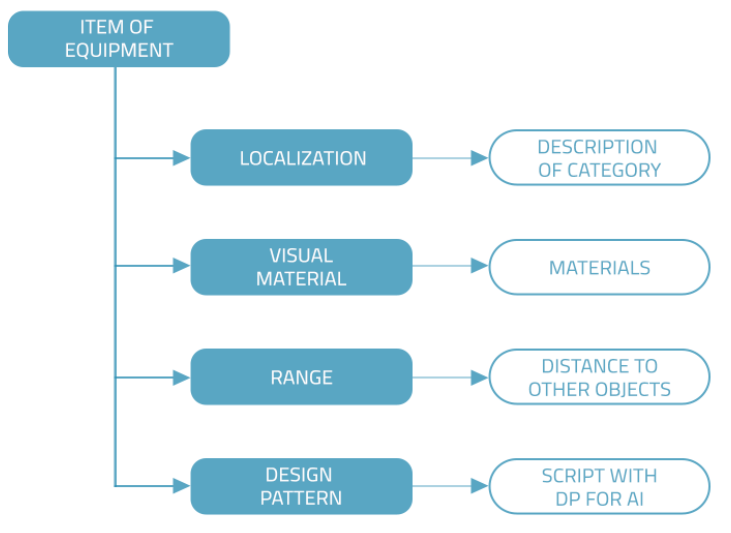
\includegraphics[width=\textwidth]{graf.png}
\caption{Types of Item of Equipment properties.} \label{fig1}
\end{figure}

Associating individual objects to categories in SADE results in assigning them independent sets of object properties (Fig. 1). Both the list of categories and properties are extensible. New categories can be added through the built-in editor, and new types of properties by adding them in individual implementations.

The example types of space categories are:
\begin{itemize}
\item bathroom
\item kitchen
\item living room
\item room
\item living room with kitchen
\item openings
\end{itemize}

Each of these space categories is associated with specific set of IoE properties. The basic types of properties are:
\begin{itemize}
\item \emph{Location} -- this property describes the specific location of a given object (a specific space category). It is important to be able to assign different locations to one object taking into account the applicable DRs without the need to multiply the element in different categories of spaces (e.g., a table may be present both in a living room and in a kitchen).\\
\item \emph{Material Identification} -- this property is used to define visual appearance of objects. Each of the materials used within an IoE can be declared as a property. Materials include elements such as color, transparency, textures, etc. The same material identification property can be assigned to multiple IoEs (e.g., glass texture can be assigned as material to both a window and the door of a shower enclosure).\\
\item \emph{Range} -- this type of property is used to define the area of impact of objects within the designed space. It contains information on the need to maintain the appropriate distance between individual objects and the empty space needed for the object. In this case, it is not possible to assign the same property to different objects due to the lack of its repeatability in DRs.\\
\item \emph{Pattern} -- this type of properties is used for the creation of sets of design rules that govern the use of this IoE. The rules defined at the IoE level are then combined with rules for ToR and general rules. 
\end{itemize}

\section{The SADE Prototype}
The SADE approach has been implemented as an Integrated Design Environment (IDE) and Shared Content Repositories (SCRs). The architecture of the SADE environment is presented in Fig. \ref{fig-arch}

\begin{figure}[H]
\centering
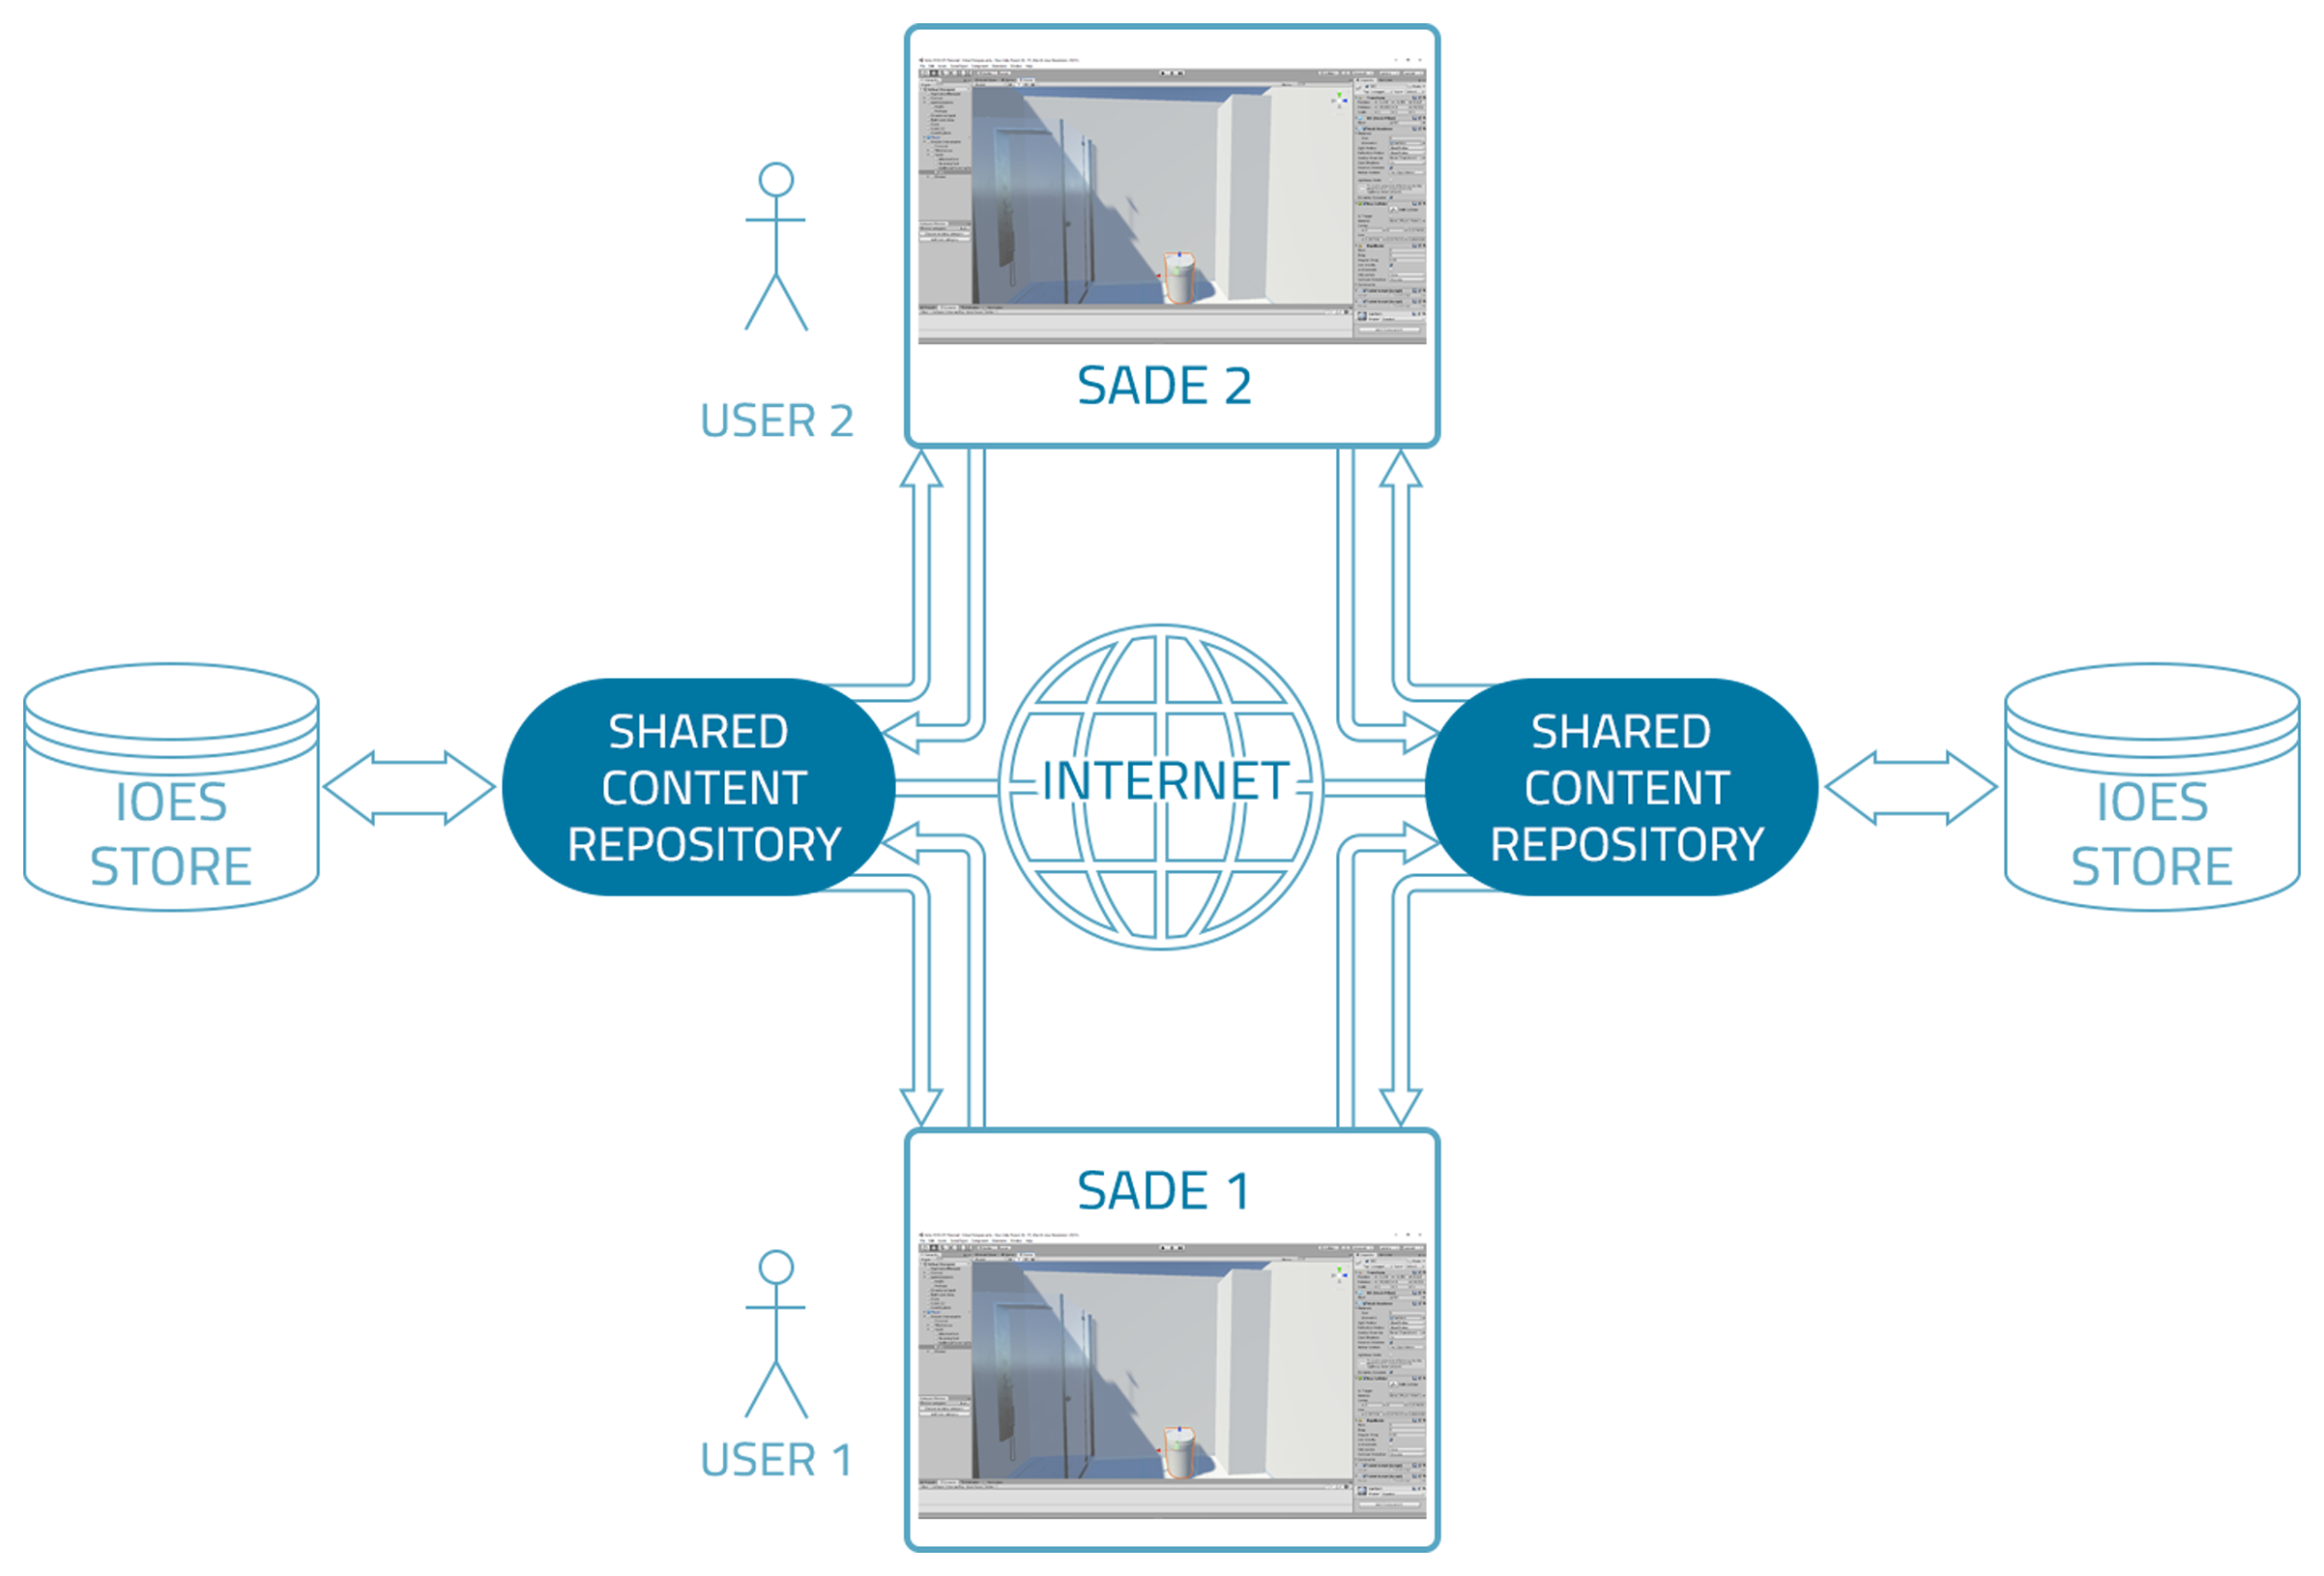
\includegraphics[width=\textwidth]{graf2.png}
\caption{Architecture of the Smart Architectural Design Environment} \label{fig-arch}
\end{figure}

The SADE environment can operate in two ways. First, it can be used as an IDE being an extension to the Unity IDE (Fig. \ref{fig-arch}), communicating with shared repositories (SCRs), which have been implemented as a REST service operating on web servers. The Unity IDE was chosen as the starting point because of its popularity and the multitude of features it has as a cross-platform gaming engine and IDE. Unity enables to freely expand the design environment with new menus, custom component editors, or editor windows using C\# and JavaScript. The SADE Unity extension enables the use of virtual rooms (ToRs) along with their IoEs, as well as creating and editing resources and sending them in parameterized form to the SCRs. This approach has been developed based on the SemFlex concept [24].

The second way of operation of the SADE environment is an application implemented in the framework of the extension that allows the use of fully immersive VR interface, in which the user has the opportunity to interact directly with the designed space. With the help of the implemented DRs, all design decisions are monitored, which enables the system to limit possible actions or inform the designer about potential design errors or non-conformities with applicable regulations.

The particular design rules are encoded in Prolog. Prolog is a declarative programming language -- the program logic is expressed in terms of relations, represented as facts and rules. It is the most popular logic programming languages, with several free and commercial implementations available. Most importantly, Prolog enables to freely combine sets of rules given that the common ontology of entities is provided. This feature enables implementation of separate sets of design rules for specific space categories in SADE, as well as combining different sources of rules: regulations, guidelines, design patterns, preferences, etc. Programming in Prolog is declarative and does not require advanced IT expertise.

An example of a set of SADE design rules programmed in Prolog is presented in Listing \ref{Script}. The rules are applicable in the bathroom context. There are six rules. The first (TD) describes the minimal and maximal distance between a toilet and a water duct. The second (TBt) describes the minimal and maximal distance between a toilet and a bathtub. The third (WmBt) describes minimal and maximal distance between a washing machine and a bathtub. Next rules describe dependencies between a washing machine and a shower, a washing machine and a sink, and a sink and a wall. All rules operate on a planar space (X,Y) assuming that the IoEs have the same vertical Z position.

For example, typically, in a bathroom almost every object position is set near a wall (e.g. toilet cannot be located in the center of the bathroom) so user has to put distance just on one of two axes -- "X" or "Y". It is also necessary to set a certain margin of error. And the last step is calculation of the distance. It is a square root of the square of the difference between the position of two objects along a given wall (in this case the "x-axis") and the perpendicular offset from it ("y-axis").\\

\begin{lstlisting}[language={c++}, caption={Example of design rules in Prolog}, label={Script}]
\end{lstlisting}

\vspace{-15pt}

\begin{footnotesize}
\begin{verbatim}
bathroomDistance_TD(T, D) :- type(T, Toilet),
			        type(D, WaterDuct),
			        (distanceXinRange(T, D, 30, 100),
			        distanceYinRange(T, D, 0, 5));
			        (distanceYinRange(T, D, 30, 100),
			        distanceXinRange(T, D, 0, 5))
			      
bathroomDistance_TBt(T, Bt) :- type(T, Toilet),
			        type(Bt, BathTub),
			        (distanceXinRange(T, Bt, 20),
			        distanceYinRange(T, Bt, 0, 5));
			        (distanceYinRange(T, Bt, 20),
			        distanceXinRange(T, Bt, 0, 5))
			      
bathroomDistance_WmBt(Wm, Bt) :- type(Wm, WashingMachine),
			        type(Bt, BathTub),
			        (distanceXinRange(Wm, Bt, 60),
			        distanceYinRange(Wm, Bt, 0, 5));
			        (distanceYinRange(Wm, Bt, 60),
			        distanceXinRange(Wm, Bt, 0, 5))

bathroomDistance_WmSh(Wm, Sh) :- type(Wm, WashingMachine),
			        type(Sh, Shower),
			        (distanceXinRange(Wm, Sh, 60),
			        distanceYinRange(Wm, Sh, 0, 5));
			        (distanceYinRange(Wm, Sh, 60),
			        distanceXinRange(Wm, Sh, 0, 5))
			      
bathroomDistance_WmSi(Wm, Si) :- type(Wm, WashingMachine),
			        type(Si, Sink),
			        (distanceXinRange(Wm, Si, 60),
			        distanceYinRange(Wm, Si, 0, 5));
			        (distanceYinRange(Wm, Si, 60),
			        distanceXinRange(Wm, Si, 0, 5))	
			        
bathroomDistance_WmSh(Si, Wa) :- type(Si, Sink),
			        type(Wa, Wall),
			        (distanceXinRange(Si, Wa, 30),
			        distanceYinRange(Si, Wa, 0, 5));
			        (distanceYinRange(Si, Wa, 30),
			        distanceXinRange(Si, Wa, 0, 5))

distanceXinRange(A, B, Min, Max) :- point(A, X1, Y1),
			        point(B, X2, Y2),
			        sqrt((X2-X1)^2 + (Y2-Y1)^2) =< Max,
			        sqrt((X2-X1)^2 + (Y2-Y1)^2) >= Min
\end{verbatim}
\end{footnotesize}

\subsection{Design example}
Creating an architectural space in SADE starts with importing a 2D projection or an empty model. A window available in the IDE menu allows the selection of categories for the Type of Room. On the left side of the application window there is a hierarchical list of elements within a given scene. At the beginning it contains only basic objects such as: Camera, Point of Light, Room Projection. In the bottom left corner of the screen located is the SADE tool window. The right side of the screen contains a preview of the created 3D scene.  When the button of an existing category is pressed, a pop-up menu appears. The list of categories is taken from a shared repository (Fig. \ref{fig-category}). After selection of the category,  a new window appears and a scalable box (Fig. 4a), by means of which the user sets the limits of a given ToR. After the user has defined the boundaries of the designed space (Fig. 4b), the actual design process begins (Fig. 5).

\begin{figure}[H]
\centering
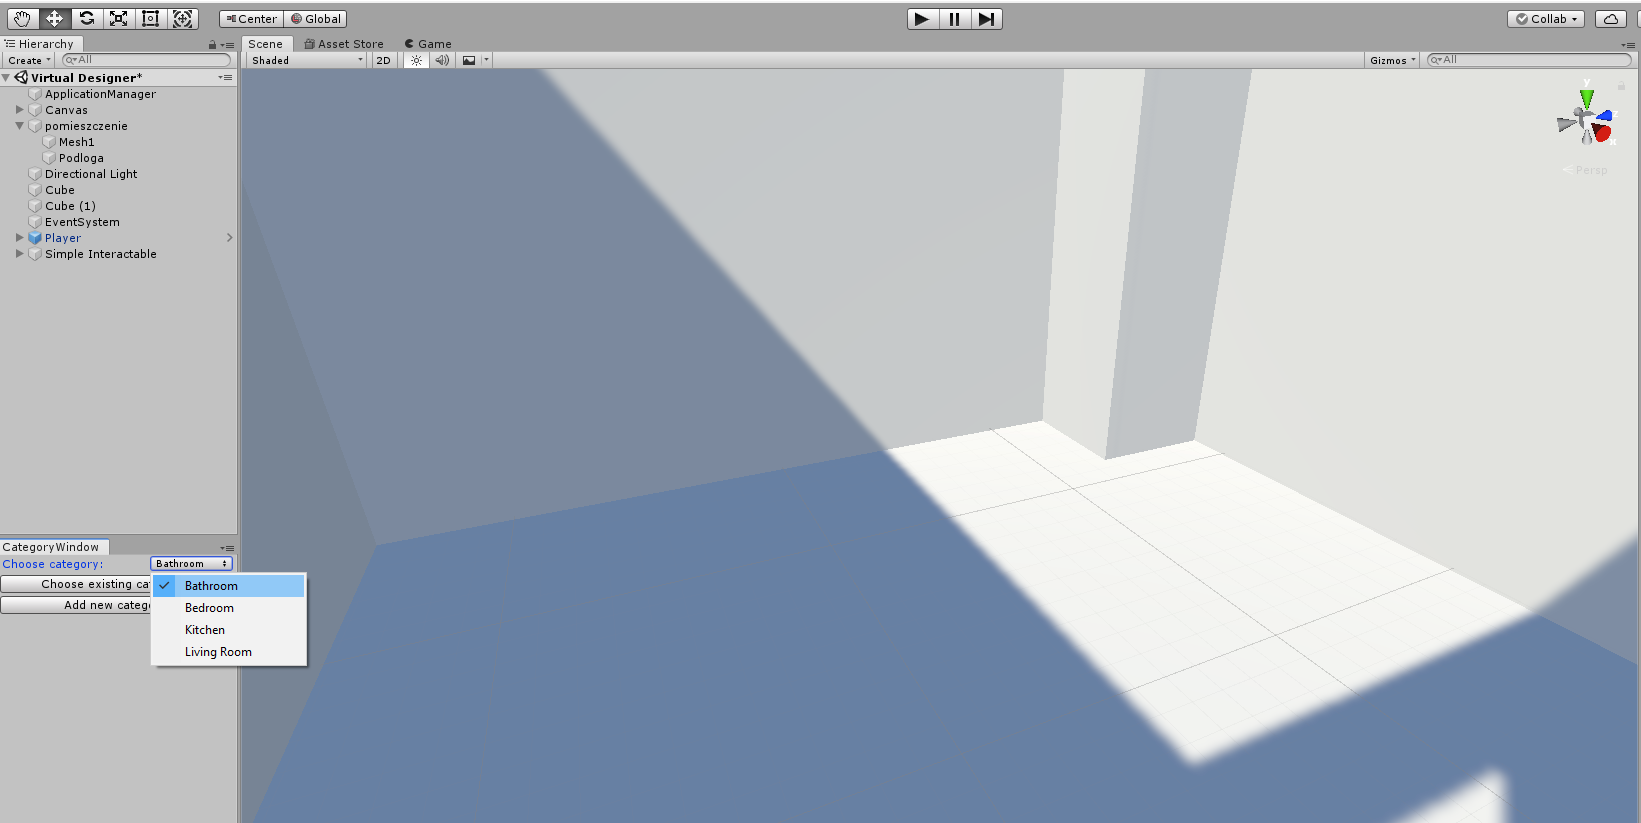
\includegraphics[width=\textwidth, height=5.3cm]{editor1.png}
\caption{Category Creator -- selection of existing ToR category} \label{fig-category}
\end{figure}

\begin{figure}
     \centering
     \subfloat[][ToR selecting window] {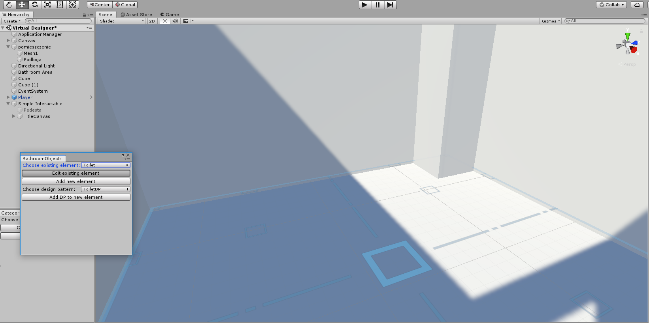
\includegraphics[width=.46\linewidth]{editor2.png}\label{fig4}}%
     \hspace{0.5cm}
     \subfloat[][ToR created and adjusted into designed space] {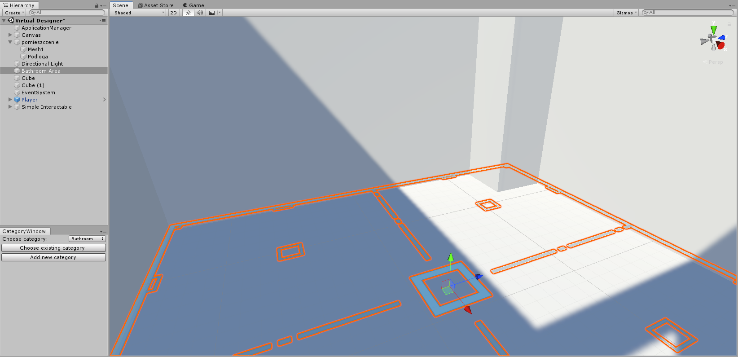
\includegraphics[width=.475\linewidth]{editor3.png}\label{fig5}}
     \caption{ToR Creator -- instantiating a Type of Room}
     \label{fig-tor}
\end{figure}

\begin{figure}[]
\centering
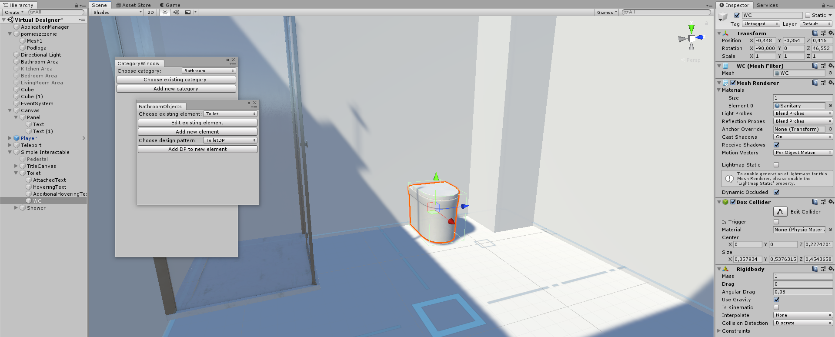
\includegraphics[width=\textwidth, height=4.55cm]{editor4.png}
\caption{Editing an Item of Equipment in SADE IDE} \label{fig6}
\end{figure}

The process consists of several phases. First of all, the designer needs to choose objects (of specific IoE category) that are to be located in the designed space. The objects are downloaded from a repository in the form of a package (.unitypackage) along with the DRs file assigned to them. After importing packages with objects, by using a drop-down menu in the application, it is possible to add individual elements to the room (washing machine, toilet, etc.). With the help of motion controllers, for example HTC Vive, the designer can interact with the objects by changing their positions, while continuously receiving feedback informing about distances from other elements contained in this space, such as shafts. 

During the design process the SADE system is continually verifying all applicable design rules. When the system identifies that the design is not consistent with the applicable design rules, the designer receives a warning about irregularities together with the considered guidelines that generate this error.

In the presented example, the room has been associated with the bathroom category, which as a room inside a flat or house has the most restrictions regarding the mutual relations between individual objects and the required distances. The design rules which have been assigned to the toilet IoE limit the distances from the duct and from the wall (Fig. 7).


\begin{figure}[]
\centering
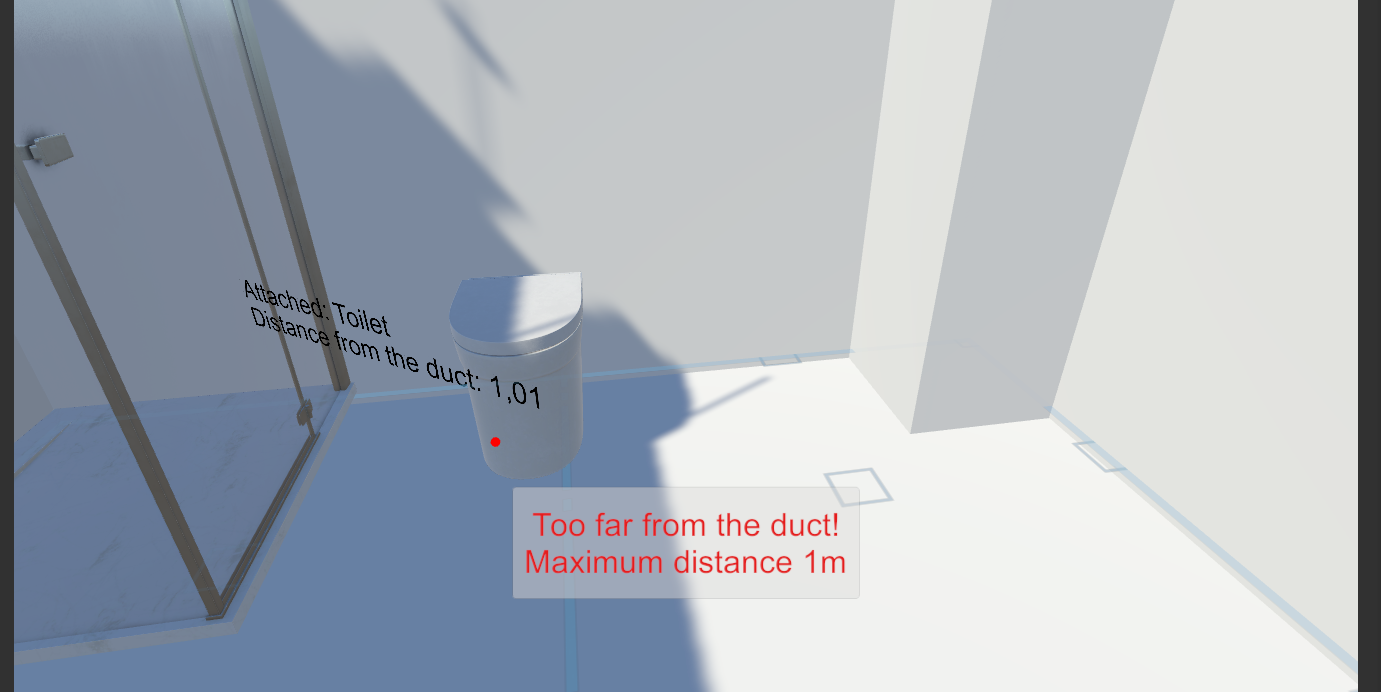
\includegraphics[width=\textwidth]{aplikacja3.png}
\caption{Displaying warning messages about mistakes made by a designer} \label{fig8}
\end{figure}

Thanks to this approach, the process of space design is simplified by limiting the choices available in a given area, which helps to avoid often obvious design mistakes, and reduces the design effort by automatic verification of rules and limiting the number of possibilities (information entropy). Thanks to the use of shared repositories, it is possible to use as components a wide range of products available on the market, and share the ready to use ToRs with other designers.


\section{Conclusions and future works}
This paper presents a new approach to the design of architectural spaces. The approach, called SADE, is based on the concept of design rules, which are formal descriptions of commonly used architectural regulations, practices, design patterns and preferences. By employing logic programming, the approach simplifies the design process, thus enabling its implementation in a fully immersive VR environment by limiting the usual complexity of this process.

Currently, the SADE IDE -- implemented as an extension to the Unity IDE -- enables creation of IoEs instances, importing content from SCRs, and creating parameterized ToRs from existing content elements. Programming of design rules is performed manually by editing the Prolog rules associated with the IoEs, ToRs as well as general rules. 

At a later stage of development, an important point to consider is creating a plug-in installed in 3D content creation programs that will enable to standardize the type of imported objects. Thanks to this, it will be possible to avoid deficiencies in export-based models. The second direction of development is to expand the system of rules to independently propose layout of elements within a given room, using typical solutions. This will allow even more simplified development of the living space. The last direction at this stage is to enable the IDE to download ready-made solutions for rooms that will only require automatic scaling and adjustment.

In future works, we plan to extend the application to support machine learning techniques, through the analysis of designers' choices and existing designs. This may further simplify the design process. 

%For citations of references, we prefer the use of square brackets
%and consecutive numbers. Citations using labels or the author/year
%convention are also acceptable. The following bibliography provides
%a sample reference list with entries for journal
%articles~\cite{ref_article1}, an LNCS chapter~\cite{ref_lncs1}, a
%book~\cite{ref_book1}, proceedings without editors~\cite{ref_proc1},
%and a homepage~\cite{ref_url1}. Multiple citations are grouped
%\cite{ref_article1,ref_lncs1,ref_book1},
%\cite{ref_article1,ref_book1,ref_proc1,ref_url1}.
%
% ---- Bibliography ----
%
% BibTeX users should specify bibliography style 'splncs04'.
% References will then be sorted and formatted in the correct style.
%
% \bibliographystyle{splncs04}
% \bibliography{mybibliography}
%
\begin{thebibliography}{8}
\bibitem{ref_art1}
Abboud R.: Architecture in an Age of Augmented Reality:  
Opportunities and Obstacles for Mobile AR in Design, Construction, and Post-Completion.  NAWIC International Women’s Day Scholarship Recipient. (2013)

\bibitem{ref_art2}
Anders, P., Lonsing, W., A.: AmbiViewer: A Tool for Creating Architectural Mixed Reality. Association for Computer Aided Design in Architecture, 104--113 (2005)

\bibitem{ref_url1}
ECMA International: Universal 3D File Format (2007) Homepagee, 
\url{http://www.ecma-international.org/}. Last accesed 7 Mar 2019

\bibitem{ref_url2}
Engineering.com: BIM 101: What is Building Information Modeling? (2016), \url{https://www.engineering.com/BIM/ArticleID/11436/BIM-101-What-is-Building-Information-Modeling.aspx}. Last accessed 7 Mar 2019

\bibitem{ref_url3}
Enscape: Homepage (2018), \url{https://enscape3d.com/architectural-virtual-reality/}. Last accessed 7 Mar 2019

\bibitem{ref_url4}
Epic Games: Unreal Engine (2019), \url{https://www.unrealengine.com/en-US/what-is-unreal-engine-4}. Last accessed 7 Mar 2019

\bibitem{ref_url5}
Eyecad VR: Homepage (2018), \url{https://eyecadvr.com/pl/}. Last accessed 7 Mar 2019

\bibitem{ref_url6}
Grasshopper Homepage, \url{https://www.grasshopper3d.com/}. Last accessed 7 Mar 2019

\bibitem{ref_url7}
IRISVR: Heomepage (2018), \url{https://irisvr.com/}. Last accessed 7 Mar 2019

\bibitem{ref_url8}
ISO. : Store - ISO 19650-1:2018 (2018), \url{https://www.iso.org/standard/68078.html}. 
Last accessed 7 Mar 2019

\bibitem{ref_url9}
ISO. : Store - ISO 19650-2:2018 (2018), \url{https://www.iso.org/standard/68080.html}. 
Last accessed 7 Mar 2019

\bibitem{ref_art3}
Kaleja P., Kozlovská M.: Virtual Reality as Innovative Approach to the Interior Designing. Selected Scientific
Papers - Journal of Civil Engineering. \textbf{12}(1), 109--116 (2017)

\bibitem{ref_url10}
Khronos Group: COLLADA - 3D Asset Exchange Schema (2017), 
\url{https://www.khronos.org/collada/}. Last accesed 7 Mar 2019

\bibitem{ref_url11}
Khronos Group: WebGL - OpenGL ES for the Web (2017), 
\url{https://www.khronos.org/webgl/}. Last accesed 7 Mar 2019

\bibitem{ref_url12}
Linkedin: 5 key differences between AutoCAD and Revit! (2017), 
\url{https://www.linkedin.com/pulse/5-key-differences-between-autocad-revit-carole-dib}. Last accessed 7 Mar 9

\bibitem{ref_art4}
Mak M.Y., Ng S.T.: The art and science of Feng Shui—a study on architects’ perception. Building and
Environment. \textbf{40}(3), 427--434 (2005)

\bibitem{ref_url13}
NEWYORK ENGINEERS: BLOG - How do AutoCad and Revit Compare? (2017), 
\url{https://www.ny-engineers.com/blog/how-do-autocad-and-revit-compare}. 
Last accessed 7 Mar 2019

\bibitem{ref_art5}
Paes D., Arantes E., Irizarry J.: Immersive environment for improving the understanding of architectural 3D
models: Comparing user spatial perception between immersive and traditional virtual reality systems.
Automation in Construction. \textbf{84}, 292--303 (2017)

\bibitem{ref_url14}
Pixel Legend: VIRTUALIST (2019), \url{https://www.pixellegend.com/virtualist/}. Last accessed 8 Mar 2019

\bibitem{ref_art6}
Portman M.E., Natapov A., Fisher-Gewirtzman D.: To go where no man has gone before: Virtual reality in
architecture, landscape architecture and environmental planning. Computers, Environment and Urban Systems.
\textbf{54}, 376--384 (2015)

\bibitem{ref_book1}
Salingaros, N. A.: Design Patterns and Living Architecture. Sustasis Press, Portland, Oregon, (2017) 

\bibitem{ref_url15}
Unity Technologies: Unity Game Engine v. 2018.3.3f1 (2018), 
\url{https://unity3d.com/unity}. Last accessed 7 Mar 2019

\bibitem{ref_url16}
VRender: Top 5 Virtual Reality Applications for Architects (2018),
\url{https://vrender.com/top-5-virtual-reality-applications-for-architects/}. 
Last accessed 7 Mar 2019

\bibitem{ref_proc1}
Walczak K.: Semantics-Supported Collaborative Creation of Interactive 3D Content. In: De Paolis L., Bourdot
P., Mongelli A. (eds.), Augmented Reality, Virtual Reality, and Computer Graphics. AVR 2017. Lecture Notes in
Computer Science, vol 10325. Springer, Cham (2017)

\bibitem{ref_art7}
Walczak, K., Cellary, W.: X-VRML for advanced virtual reality applications. Comput.
 \textbf{36}(3), 89--92 (2003)

\bibitem{ref_art8}
Walczak, K., Wojciechowski, R., W\'{o}jtowicz, A.: Interactive production of dynamic
3D sceneries for virtual television studio. -In: The 7th Virtual Reality IC VRIC -
Laval Virtual, pp. 167--177, Laval (2005)

\bibitem{ref_art9}
Wang X.: Augmented Reality in Architecture and Design: Potentials and Challenges for Application.
International journal of architectural computing. \textbf{02}(7), 309--326 (2009)

\bibitem{ref_url17}
Web3D: The Virtual Reality Modeling Language - ISO/IEC 14772–1 (2006).
\url{http://www.web3d.org/standards/all}. Last accesed 7 Mar 2019

\bibitem{ref_url18}
Web 3D: X3D Specifications - ISO/IEC-19775-1 (2013), 
\url{http://web3d.org/x3d/specifications/}. Last accessed 7 Mar 2019

\end{thebibliography}
\end{document}
